\chapter{Introduction}
\label{introduction}

\renewcommand{\thepage}{\arabic{page}} 			% arabic enumeration
\setcounter{page}{1}                   			% set page number 1

In these last years, a growing interest has been shown in robotics. In fact, several industries (automotive, medical, manufacturing, space, etc.), require robots to replace men in dangerous, repetitive or onerous situations. A wide area of this research is dedicated to Unmaned Aerial Vehicle (UAV) and especially the one of having the capability of Vertical TakeOff and Landing (VTOL) \cite{largeQuadrotor}. This kind of vehicle can be use in a variety of different scenario, for its reasonable price, small dimensions and great sensors capability. In particular, nowdays intensive research as been accomplish in the area of enviroment monitoring and exploration, perform with different strategies and sensors.

\begin{SCfigure}[\sidecaptionrelwidth][h]
	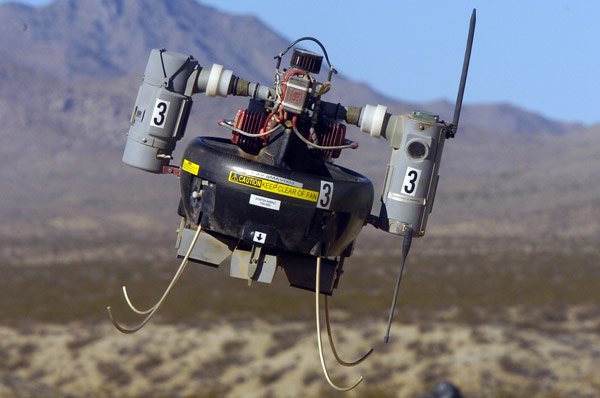
\includegraphics[scale=0.4]{images/fukushima.jpg}
	\caption{An example of UAV. T-Hawk, a US-made UAV, commonly used to search for roadside bombs in Iraq, made its debut when it photographed the Fukushima nuclear plant from above, providing a detailed look at the interior damage.}
	\label{fig:application}
\end{SCfigure}  

\noindent Many typse of UAVs have been developed over the last years, in particular the quadrotor type \cite{Aalborg}. The aim of this thesis is to contribute the develop of the so called \textit{Prometheus mapping drone}, a fully autonomus vertical takeoff and landing vehicle, able to perform indoor enviroment exploration and mapping. To do this, we were inspired from the film Prometheus, where drones are able to map an indoor cave. Of course, due to technology and budget limitations, the vehicle will not have the same performance, but will have in theory the same capabilities. As previously said, this thesis is only a part of the project, that has been divided in three main parts:

\begin{itemize}
	\item mechanical design and building of the UAV \cite{Carlos};
	\item mathematical model, system identification and control;
	\item usage of the sensors, mapping and navigation algorithms.
\end{itemize}

\noindent This thesis will focus on the second point, mathematical model, system identification and control, but briefly introductions will give also in the other two points, in particular in the mechanical design, necessary for develop a mathematical model. 

\begin{SCfigure}[\sidecaptionrelwidth][h]
	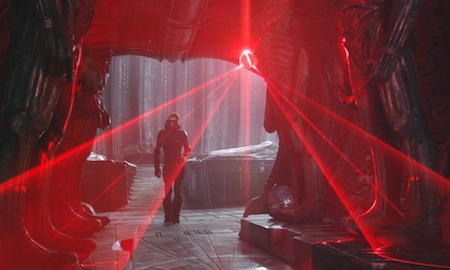
\includegraphics[scale=0.6]{images/prometheus_film.jpg}
	\caption{Frame of the prometheus movie, where the drone is performing the exploration and mapping of the cave.}
	\label{fig:prometheusFILM}
\end{SCfigure}

\begin{SCfigure}[\sidecaptionrelwidth][h]
	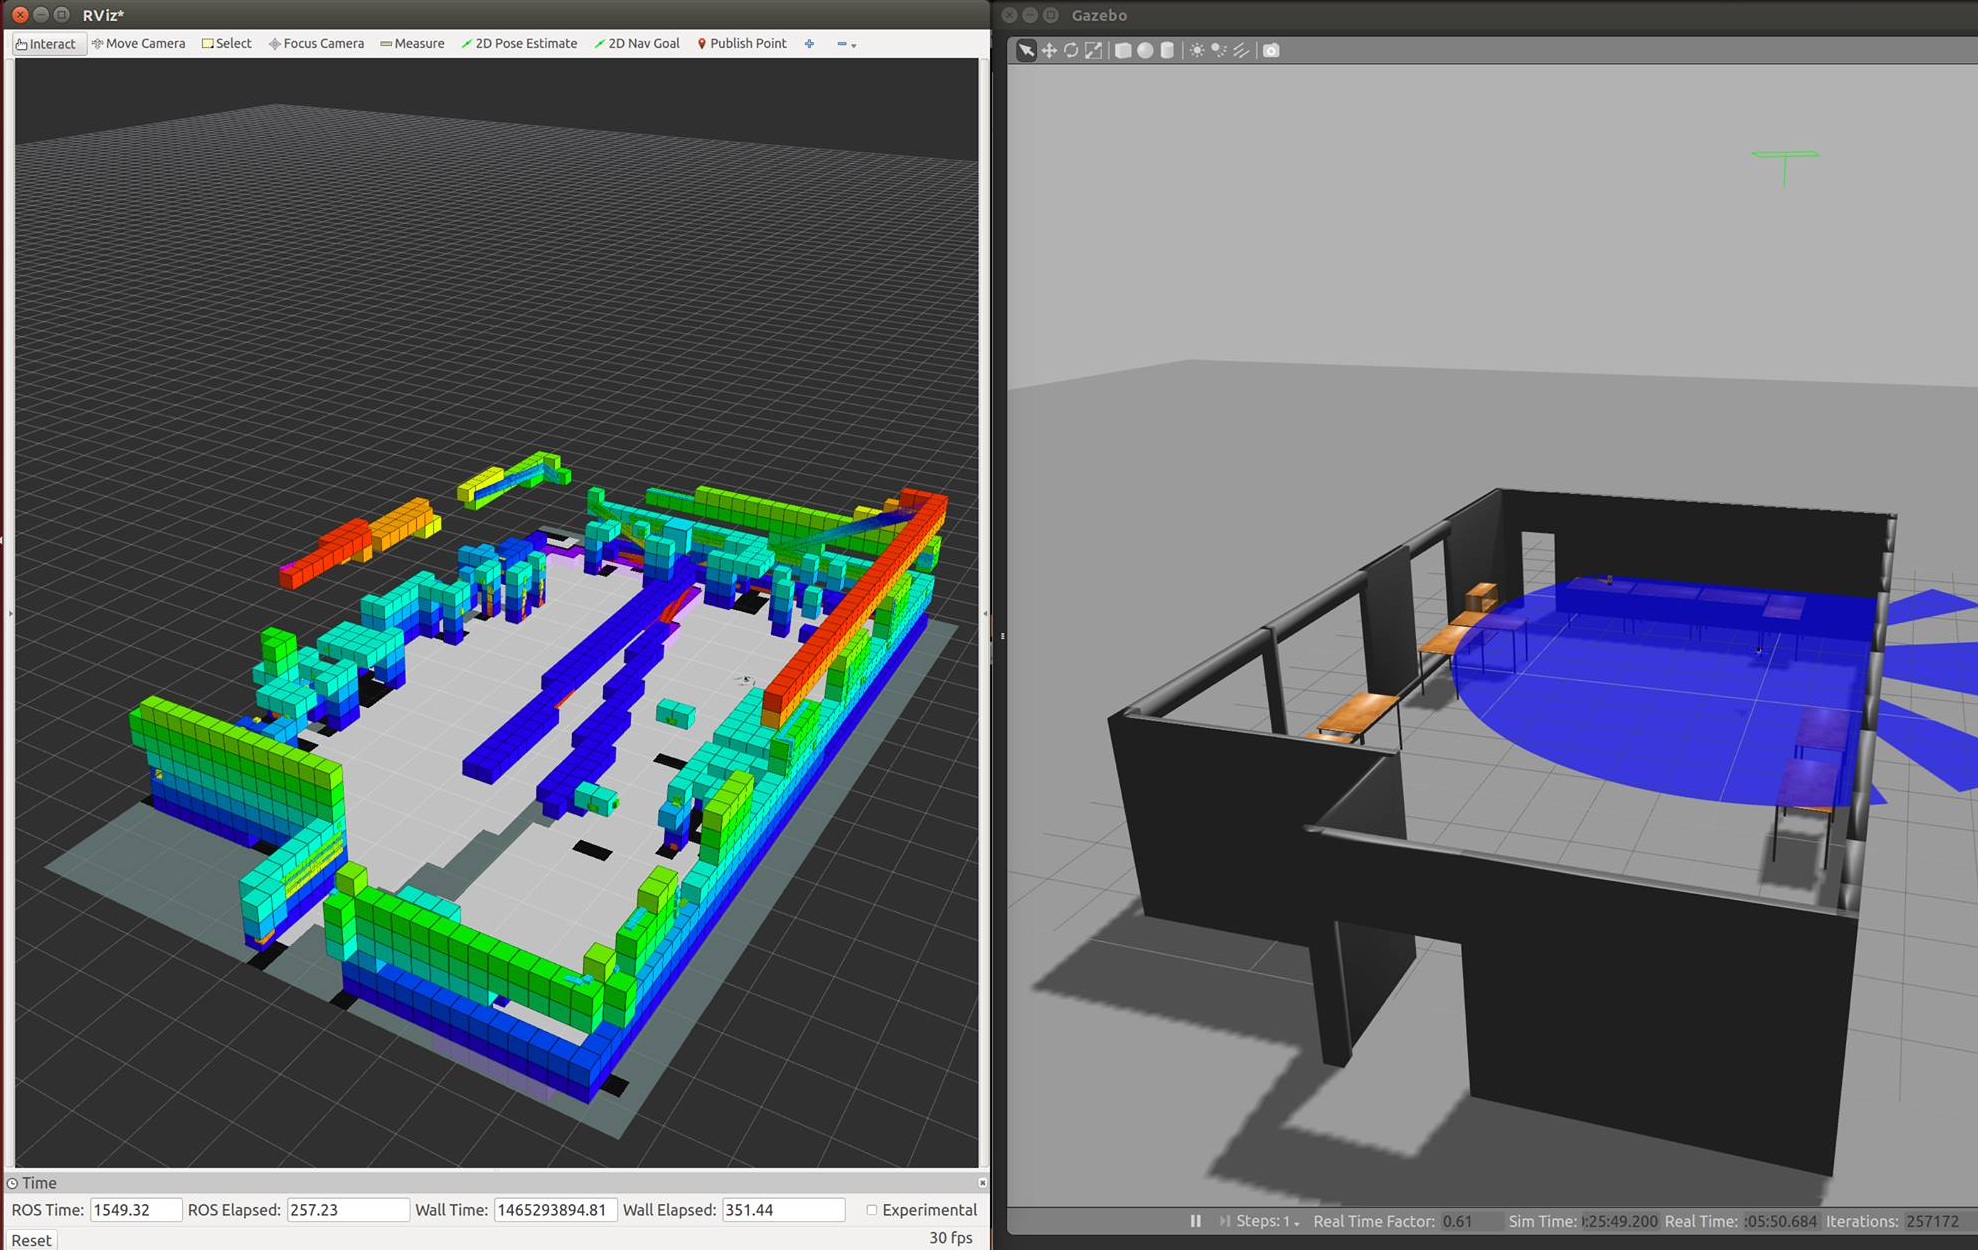
\includegraphics[scale=0.1364]{images/simulation_Romain.png}
	\caption{Simulation of the navigation and mapping from the third point of this thesis.}
	\label{fig:simulationRomain}
\end{SCfigure}

\noindent In details, this thesis is divided in differnt chapters.

\noindent In chapter \ref{designModel} we will discus about the mechanical design of the UAV, the sensors used and the reasons for it. From this, a mathematical model will be derive, complete with all the notation and math needed to describe the dynamic of the vehicle. Of course, reasonable simplifications will be perform on the way. Then we will describe the experimental setup, with all the hardware and software used for this project.

\noindent In chapter \ref{systemIdentification} we will perform the system identification of the parameters of the UAV. Before doing it, we will do simplification of the system, just to reduce the number of the parameters and especially to linearize it. The reason to linearize the system, introducing some errors, is because we choose to use a standerd Kalman filter approach to the system identification problem. With this approach we will see that all the parameters will be estimated.

\noindent In chapter \ref{trajectoriesGenerator} a trajectories generator algorithm will be describe. This is necessary because usually, path finding and navigation algorithms provides only setpoint and not full trajectory that smootly connect the different setpoints. We will describe a trajectory generator that smootly connects setpoint till the fourth derivative of the position, the so called snap. Moreover, corridor constraints will be added to the problem. A corridor constraint takes into account that the trajectory must be inside a virtual corridor between two setpoints. This because if we not impose any constraints we van end up with a trajectory that actually connects different setpoints, but maybe hit a wall. This is extrimily important, since our main goal is to operate the vehicle in a indoor environment. 

\noindent In chapter \ref{control} we will talk about the control of the vehicle. For control we mean that the UAV must follow the desire trajectory in the space with the minimum error. This control will take into account also the particular structure of the drone. It will be derive from the mathematichal model describe previously.

\noindent In the end, in chapter \ref{conclusions} we will draw the conclusions of this work. Moreover, we will describe also future possible works, that start from some consideration of this thesis. 